\documentclass[12pt]{report}
\usepackage{amsmath,amssymb,amsfonts}
\usepackage{courier}
\usepackage{graphicx}
\usepackage{hyperref}
\usepackage{listings}
\usepackage{color}
\usepackage{tikz}
\usepackage{circuitikz}
\usetikzlibrary{shapes,arrows}
\usepackage[margin=2cm]{geometry}

\title{ECSE 426 - Microprocessor Systems\\Lab Report 2: Timers, Interrupts, Multithreaded, Interrupt-Driven Readings and Peripheral Control}
\author{Harley Wiltzer (260690006)\\Matthew Lesko (260692352)}
\date{March 19, 2018}

\definecolor{dblue}{rgb}{0.4,0.4,0.8}

\hypersetup {
	colorlinks=true,
	linkcolor=dblue
}

\tikzstyle{decision} = [diamond, draw, fill=blue!20, text badly centered, text width=2cm, node
distance=3cm]
\tikzstyle{block} = [rectangle, draw, fill=blue!20, text centered, rounded corners, minimum
height=4em, text width=3cm, node distance=5cm]
\tikzstyle{goal} = [rectangle, draw, fill=yellow!20, text centered, rounded corners, minimum
height=4em, text width=3cm, node distance=5cm]
\tikzstyle{line} = [draw, -latex']
\tikzstyle{cloud} = [draw, ellipse, fill=red!20, node distance=7cm, text centered, text width=2cm]
\tikzstyle{label} = [draw, rectangle, text centered, text width = 3cm]

\renewcommand*\thesection{\arabic{section}}

\begin{document}
\maketitle
\pagenumbering{roman}
\tableofcontents
%\let\clearpage\relax
\listoffigures
\let\clearpage\relax
\listoftables
\newpage
\pagenumbering{arabic}
\section{Abstract}
The purpose of experiment 3 is for the programmers to gain experience in utilizing timers and interrupts to accomplish a task which involves converting an analog pulse to digital and displaying its voltage on an LED display, effectively a voltmeter. The purpose of experiment 4 is for the programmers to gain exposure in designing a multithreaded program on a real time operating system (RTOS) running on an embedded system. The task of experiment 4 involves copying over experiment 3's program and subdiving several of its features each to its own concurrently running thread, with the goal of optimizing power usage. This report will explain in detail how the programmers implemented the problems stated below, as well as the challenges they faced, the testing they had done, and the conclusions they have made. By the end of the report, the reader shall understand how the timers available on the STM32F4 board can be used to activate peripherals and generate a pulse, and understand the implementation of multithreaded programs on embedded systems.
\section{Problem Statement}
The problem is for the developers to first implement a solution for generating a PWM pulse, whose voltage is set by an input on a keypad, that is then fed to a rectifier. Afterwards, the device shall feed the rectifier's output to an ADC to be converted to a digital signal, and have the signal's mean voltage be automatically displayed on an LED display. Furthermore, the program has to be implemented with the use of concurrently-running threads running on an RTOS. The problem can be divided into the following tasks:
\begin{itemize}
	\item Setting up a timer to act as a PWM pulse generator;
	\item Setting up a timer to activate the ADC to take an analog sample and convert it to digital;
	\item Designing a rectifier circuit component that takes the PWM pulse as input and feeds the output to the ADC;
	\item Testing and optimization of an FIR filter that reduces noise from the output signal of the ADC;
	\item Setting up the alphanumeric keypad so that the user may input their desired voltage to be displayed on an LED display;
	\item Mainting the 7-segment display;
	\item Coding a controller function that automates the changes to be made on the PWM's duty cycle so that the previous or default voltage updates to the target voltage on the LED display;
	\item Coding a finite state machine function that enables the user to Enter and Delete digits for the target voltage, Reset the target voltage, and put the device to Sleep by using the keypad;
	\item Implementing the program's features using CMSIS-RTOS and multithreading;
	\item Reducing the power consumption of the device when it is in sleep mode using CMSIS-RTOS.
\end{itemize}
\section{Theory and Hypothesis}
Since this experiment uses components from experiment number 2, any theory for the identical components that has been mentionned in the previous lab report will be skipped. If you need to see theory for those components, and it is not mentionned here, please refer to Lab Report number 1.

\subsection{Rectifier}
A rectifier is a component that converts alternating current (AC) to direct current (DC). It does so by only allowing a one-way flow of electrons, by the use of a diode. The diode allows electric current only in the forward bias condition and blocks electric current in reverse bias condition, this allows it to act like a rectifier. The output of the diode only contains a positive half cycle, as opposed to the input having a positive and a negative half cycle [1]. The rectifier component of this experiment's device contains a diode connected in series with a parallel connection of a resistor and a capacitor.

\subsection{Multithreading and Semaphores}
The idea of multithreading is to have multiple threads execute concurrently. This allows for parallelism, more effecient use of a processor, and faster execution time. This is similar to the notion of concurrently-running processes, however, threads are not processes. One can have multiple threads running in one process, thus allowing for less overhead because the threads all share the same data [2]. Since, the threads may be sharing resources, this requires some kind of mutual exclusion to prevent threads from falling into deadlock or race-condition situations. The solution is semaphores. Semaphores allow one program to use a shared resource without having other programs use the resource at the same time. This is done by having a program wait until a semaphore is available to use before it can have access to the shared resource and execute its code. First a program waits for a semaphore, and once it is available, holds the semaphore by decrementing the semaphore's count, and executing its code. If the semaphore has a value of 0, no other program that is waiting for the same semaphore can execute. When the program using the shared resource no longer has need for the resource, it releases the semaphore by incrementing the semaphore's count, thus allowing other programs that are waiting to execute, to use the resource [2]. This resolves the problem of deadlocks and race-conditions.

\subsection{Hypothesis}
The programmers should be able to implement a solution for experiment 3 given the time allocated for the project. The challenges one expects to face are learning how to use the keypad and implementing a solution with it, testing of the resistor and capacitor components for the rectifier, and implementing a solution for the different features available on the keypad with the use of a finite state machine. The programmers should be able to implement a solution for experiment 4 given the time allocated for the project, since the majority of the device and code is the same from experiment 3 and the students should have had experience with multithreading and semaphores.

\section{Implementation}

\subsection{PWM Pulse Generation}
The developers were tasked with designing a system that generates PWM pulses and feeds the voltage to a rectifier circuit. Under the \hyperref[appendixtim2]{TIM3 configuration settings}, a timer, one can see that it is configured to generate a pulse at a frequency of 1MHz, by inheriting the system's clock of 168MHz and having a period of 168, hence having 168 MHz divided by 168, yielding 1 MHz. The students have chosen to use this frequency after having tested lower frequencies, and came to the conclusion that in order for the duty cycle to control the output voltage, the frequency had to be elevated to at least this amount of frequency. After \hyperref[testpwm]{testing and observing}, the students noticed that a frequency of 1 MHz was suitable enough to have the duty cycle control the output voltage. The STM32F4's TIM3 hardware timer is configured to generate and output a PWM pulse channel that is assigned to a GPIO pin on the board, which can be viewed in the \hyperref[pinconfig]{GPIO pin configuration table} generated by STMCubeMX. By using a circuit wire, the programmers can feed the output of the PWM pulse channel to a circuit component on a bread board, more specifically, the rectifier.\\
The rectifier circuit holds the charge in the capacitor while a load resistance discharges the capacitor, enabling the user to influence the duty cycle to control the output voltage level. The required range for the output voltage is between 0.5V and 2.8V, hence it is required to test different configurations for the resistor and capactitor to deliver a range of output voltages that meet the requirement. The students have chosen a capacitor of 5uF and a resistor of 390 Ohms. This configuration was chosen because it achieved an output voltage range of 0.4V to roughly 2.1V. The programmers were able to observe this phenomenon after \hyperref[testpwm]{testing} multiple different configurations and came to the conclusion that the resistor and capacitor values chosen were suitable for the task.

\subsection{ADC and Timers}
Previously, the students used STM's built-in SysTick to enable the ADC. For this experiment, the students had configured the ADC to be triggered by an STM32F4 timer, specifically TIM2. Under the \hyperref[appendixtim2]{TIM2 configuration settings}, one can see that the timer is configured with a prescaler of 83999 and a period of 1, which by inherting the system clock of 168 MHz, entails the timer to a frequency of 500 Hz. The reason behind this decision is so that the ADC gets activated frequently enough to take samples more often. This would allow it to be a more responsive component and allow the output voltage's RMS to be updated more accurately. One can see under the \hyperref[appendixadc]{ADC's configuration settings} that the trigger for the ADC's activation is the TIM2's trigger event.

\subsection{Filtering}
The devices uses a modified FIR filter from experiment 2 in order to reduce the noise of the ADC's signal. The two modifications are the following: 
\begin{itemize}
	\item Increasing from 5 coefficients to 10 being used in the moving average;
	\item Setting the first five coefficients to 0.05 and the last five coefficients to 0.15.
\end{itemize}
In this way, the 5 earliest samples hav have a significance of 0.05 and the 5 later samples have a significance of 0.15 when calculating the average of the 10 samples. The programmers drew this conclusion by trial and error and the empirical evidence proved that the above modifications to the FIR filter significantly reduced the signal's noise. The programmers have tested mutliple configurations, in which this report shall demonstrate three of the tested configurations. The graphs the programmers have used to determine the optimized filter can be seen in the  \hyperref[testfiltering]{Testing and Observations: Filtering}, section. After testing multile configurations, the three that are graphed in the testing section further prove that the programmers have chosen an accurate filter with coefficients: [0.15, 0.15, 0.15, 0.15, 0.15, 0.05, 0.05, 0.05, 0.05, 0.05].

%TODO These sections
\subsection{Alphanumeric Keypad}


\subsection{Finite State Machine}


\subsection{Controller}

\subsection{Multithreading}

\section{Testing and Observations}

\subsection{PWM and Rectifier}\label{testpwm}

The students tested multiple configurations of resistor and capacitor values for the rectifier circuit. Here were their findings:\\

\textbf{Duty Cycle VS Output Mean Voltage}\\
	Resistor: 4.7K Ohms, Capacitor: 20 uF\\
	\begin{tabular}{|c|c|}
		\hline
		Duty Cycle & Output Mean Voltage (V)\\\hline
		0.05 & 1.620\\\hline
		0.95 & 2.150\\\hline
	\end{tabular}
	\newline
	\\
\textbf{Duty Cycle VS Output Mean Voltage}\\
	Resistor: 4.7K Ohms, Capacitor: 5 uF\\
	\begin{tabular}{|c|c|}
		\hline
		Duty Cycle & Output Mean Voltage (V)\\\hline
		0.05 & 1.600\\\hline
		0.95 & 2.140\\\hline
	\end{tabular}
	\newline
	\\
\textbf{Duty Cycle VS Output Mean Voltage}\\
	Resistor: 390 Ohms, Capacitor: 20 uF\\
	\begin{tabular}{|c|c|}
		\hline
		Duty Cycle & Output Mean Voltage (V)\\\hline
		0.05 & 0.364	\\\hline
		0.95 & 1.920\\\hline
		1.00 & 1.920\\\hline
	\end{tabular}
	\newline
	\\
\textbf{Duty Cycle VS Output Mean Voltage}\\
	Resistor: 390 Ohms, Capacitor: 5 uF\\
	\begin{tabular}{|c|c|}
		\hline
		Duty Cycle & Output Mean Voltage (V)\\\hline
		0.05 & 0.401	\\\hline
		0.95 & 1.930\\\hline
		1.00 & 2.105\\\hline
	\end{tabular}
	\newline
	\\
One can see that having a small resistor (390 Ohms) and low capacitor (5uF) allow the output voltage to yield a range roughly between 0.4V and 2.1V, making it the best suitor for the requirement of delivering a wide range of output voltages. Since the resistor used is small, adding a resistor in parallel as the load resistor won't affect the circuit unless it is as small as the 390 Ohm resistor.

\subsection{Filtering}\label{testfiltering}
One can draw comparisons from the following graphs generated by a run-time variables monitoring and visualization tool, STM Studio [source]:\\
\begin{figure}[h] % TODO: i want my graph between the two blocks of text
	\label{Linear Graph of the Filtered and Unfiltered Values Plotted Against Time}
	\begin{center}
		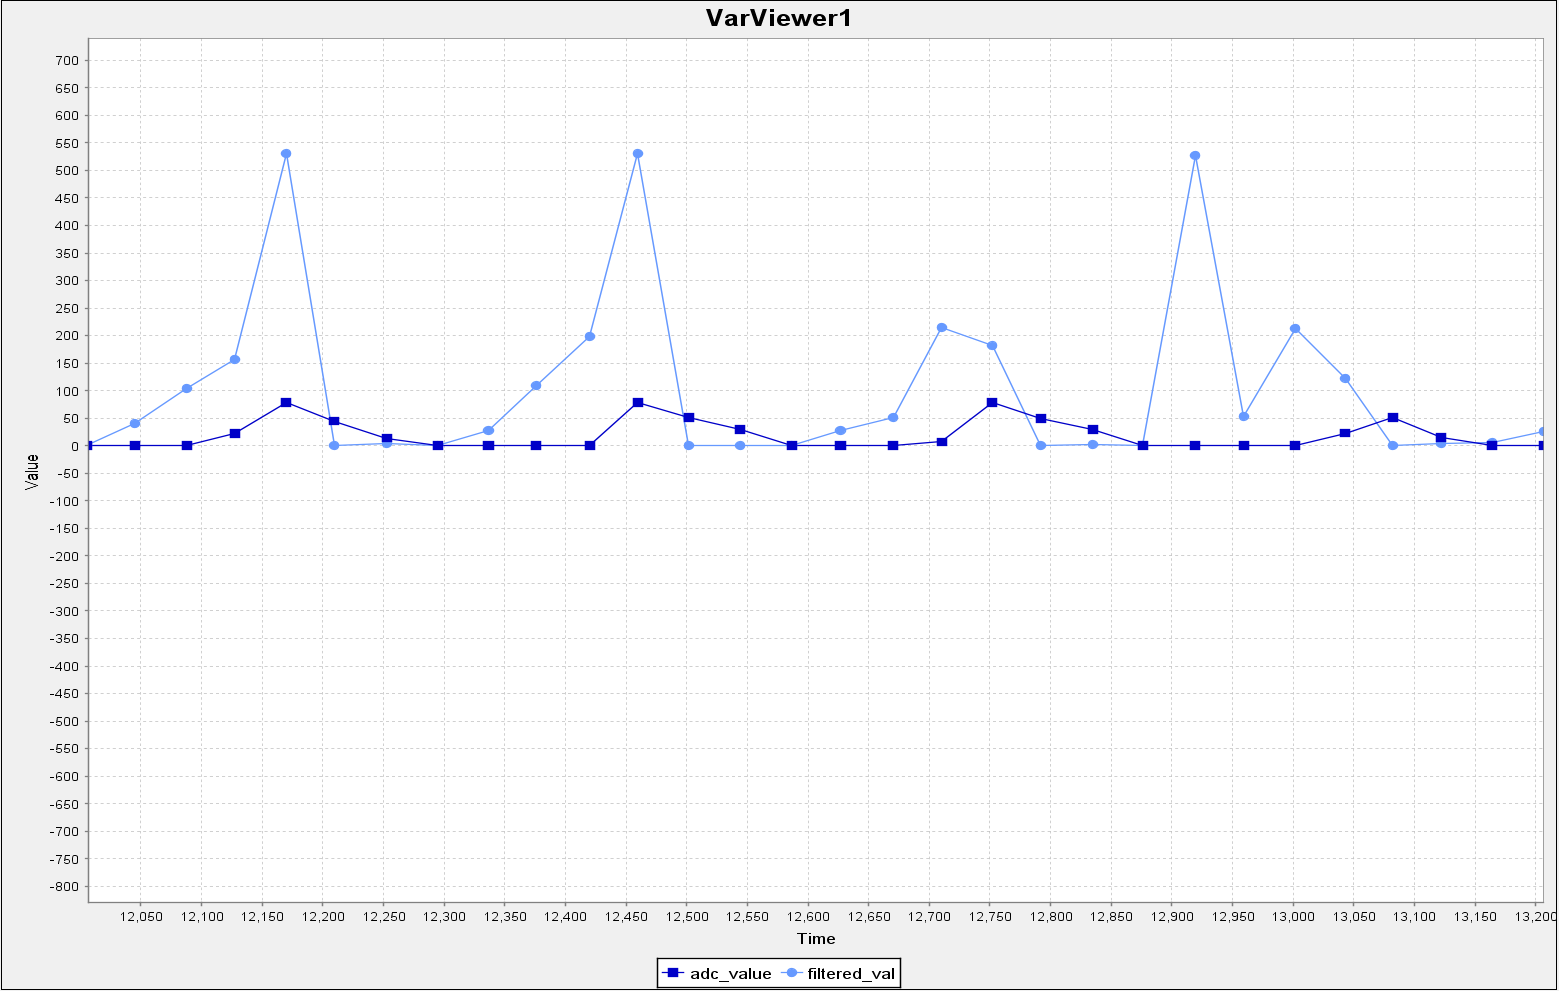
\includegraphics[scale=0.5]{./figures/adc_5coeffs.PNG}
		\caption{Filtered and Unfiltered Values VS Time (ms), Using Unmodified FIR Filter}
	\end{center}
\end{figure}
\\For the graph above, the configuration for the filter's coefficients is [0.2, 0.2, 0.2, 0.2, 0.2]. In regular blue are the unfiltered values, and in light blue are the filtered values. This graph demonstrates the values read at runtime of the unfilted and filtered values that passed through the unmodified FIR filter. One can observe that there is a considerable amount of noise left from filtering.
\begin{figure}[h] % TODO:  i want my graph between the two blocks of text
	\label{Linear Graph of the Filtered and Unfiltered Values Plotted Against Time}
	\begin{center}
		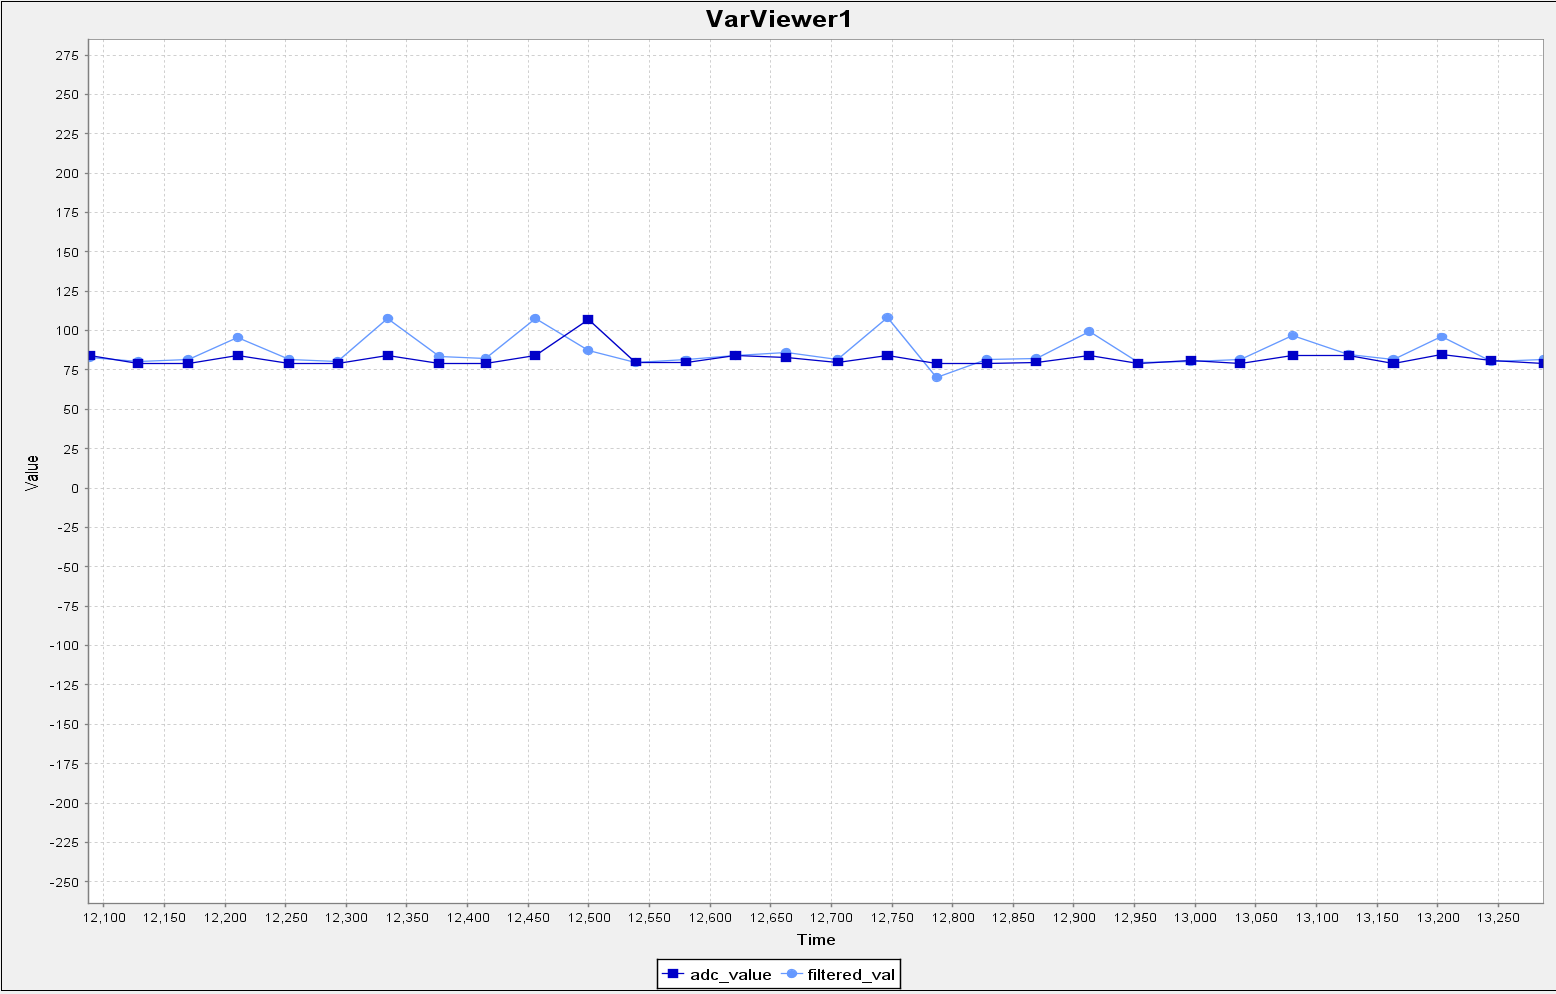
\includegraphics[scale=0.5]{./figures/adc_10coeffs_early_high_values.PNG}
		\caption{Filtered and Unfiltered Values VS Time (ms), Using High Coeffcients for Early Values}
	\end{center}
\end{figure}
\\For the graph above, the configuration for the filter's coefficients is [0.05, 0.05, 0.05, 0.05, 0.05, 0.15, 0.15, 0.15, 0.15, 0.15]. This filter considers the five earliest values to each have a significance of 0.15 and the five later values to each have a significance of 0.05. One can observe by the graph that this filter is a considerable improvement to the unmodified version. Although, the programmers believe that it could be optimized further.
\begin{figure}[h] % TODO:  i want my graph between the two blocks of text
	\label{Linear Graph of the Filtered and Unfiltered Values Plotted Against Time}
	\begin{center}
		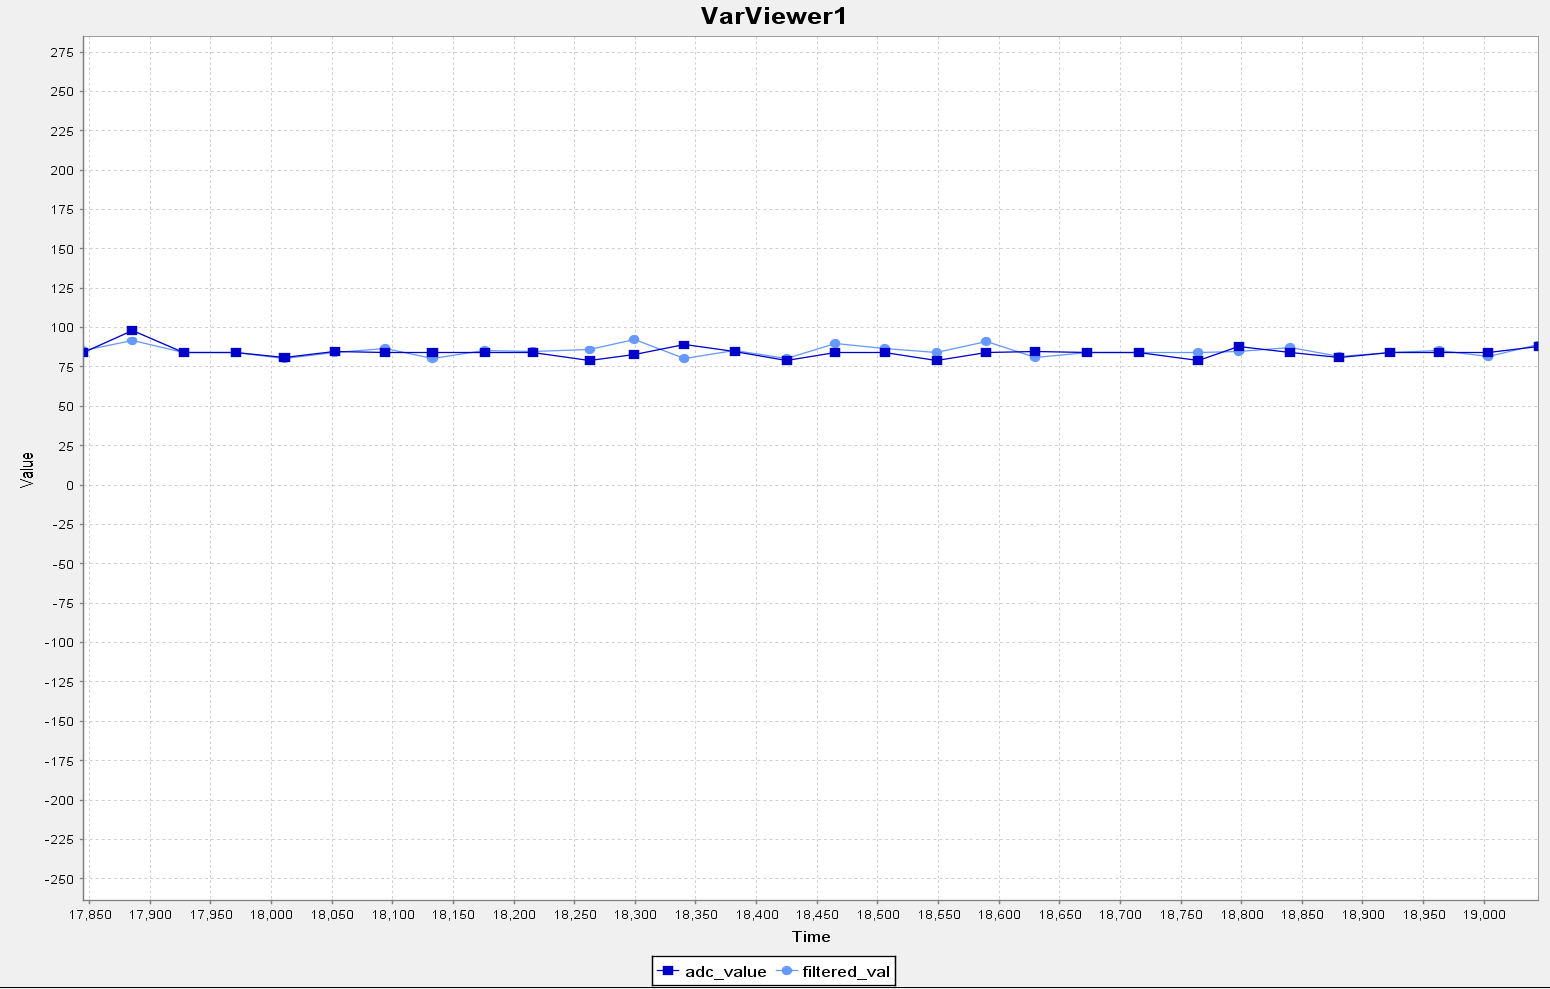
\includegraphics[scale=0.5]{./figures/adc_10coeffs_late_high_values.PNG}
		\caption{Filtered and Unfiltered Values VS Time (ms), Using High Coeffcients for Late Values}
	\end{center}
\end{figure}
\\For the graph above, the configuration for the filter's coefficients is [0.15, 0.15, 0.15, 0.15, 0.15, 0.05, 0.05, 0.05, 0.05, 0.05]. This filter considers the five later values to each have a significance of 0.15 and the five early values to each have a significance of 0.05. One can observe by the graph that this filter is an improvement to the previous version. The programmers believe that this version of the filter should perform well enough given the scope of the problem.

\section{Conclusion}
\newpage
\begin{appendix}\label{appendices}
	\chapter{GPIO Configuration Parameters}\label{appendixgpio}
	This appendix lists the configuration parameters set for each of the different GPIO pins (or
	classes of GPIO pins).\\\\
	\textbf{User Input Button}\\
	\begin{tabular}{|c|c|}
		\hline
		Parameter & Value\\\hline
		Mode & \texttt{GPIO\_MODE\_IT\_RISING}\\\hline
		Pull & \texttt{GPIO\_NOPULL}\\\hline
	\end{tabular}
	\newline
	\\\\
	\textbf{Display Mode LEDs (4 of these)}\\
	\begin{tabular}{|c|c|}
		\hline
		Parameter & Value\\\hline
		Mode & \texttt{GPIO\_MODE\_OUTPUT\_PP}\\\hline
		Pull & \texttt{GPIO\_NOPULL}\\\hline
		Speed & \texttt{GPIO\_SPEED\_FREQ\_LOW}\\\hline
	\end{tabular}
	\newline
	\\\\
	\textbf{Display Segment Pins (8 of these)}\\
	\begin{tabular}{|c|c|}
		\hline
		Parameter & Value\\\hline
		Mode & \texttt{GPIO\_MODE\_OUTPUT\_PP}\\\hline
		Pull & \texttt{GPIO\_NOPULL}\\\hline
		Speed & \texttt{GPIO\_SPEED\_FREQ\_LOW}\\\hline
	\end{tabular}
	\newline
	\\\\
	\textbf{Display Selector Pins (3 of these)}\\
	\begin{tabular}{|c|c|}
		\hline
		Parameter & Value\\\hline
		Mode & \texttt{GPIO\_MODE\_OUTPUT\_PP}\\\hline
		Pull & \texttt{GPIO\_NOPULL}\\\hline
		Speed & \texttt{GPIO\_SPEED\_FREQ\_LOW}\\\hline
	\end{tabular}
	\newline
	\newpage
	\chapter{ADC Configuration Settings}\label{appendixadc}
	\textbf{ADC Instance Parameters}\\
	\begin{tabular}{|c|c|}
		\hline
		Parameter & Value\\\hline
		Clock Prescaler & \texttt{ADC\_CLOCK\_SYNC\_PCLK\_DIV4}\\\hline
		Resolution & \texttt{ADC\_RESOLUTION\_8B}\\\hline
		Scan Conversion Mode & Disabled\\\hline
		Continuous Conversion Mode & Disabled\\\hline
		Discontinuous Conversion Mode & Disabled\\\hline
		External Trigger Conversion Edge & \texttt{ADC\_EXTERNALTRIGCONVEDGE\_RISING}\\\hline
		External Trigger Conversion & \texttt{ADC\_EXTERNALTRIGCONV\_T2\_TRGO}\\\hline
		Data Alignment & \texttt{ADC\_DATAALIGN\_RIGHT}\\\hline
		Number of Conversions & 1\\\hline
		DMA Continuous Requests & Disabled\\\hline
		EOC Selection & \texttt{ADC\_EOC\_SINGLE\_CONV}\\\hline
	\end{tabular}
	\newline
	\\\\
	\textbf{ADC Channel Parameters (Channel 1)}\\
	\begin{tabular}{|c|c|}
		\hline
		Parameter & Value\\\hline
		Rank & 1\\\hline
		Sampling Time & \texttt{ADC\_SAMPLETIME\_28CYCLES}\\\hline
	\end{tabular}
	\newpage
	
	\chapter{TIM2 Configuration Settings}\label{appendixtim2}
	\textbf{TIM2 Instance Parameters}\\
	\begin{tabular}{|c|c|}
		\hline
		Parameter & Value\\\hline
		Instance & \texttt{TIM2}\\\hline
		Clock Prescaler & \texttt{83999}\\\hline
		Counter Mode & \texttt{TIM\_COUNTERMODE\_UP}\\\hline
		Period & 1\\\hline
		Clock Division & \texttt{TIM\_CLOCKDIVISION\_DIV1}\\\hline
	\end{tabular}
	\newline
	\\\\
	\textbf{TIM2 Clock Source Parameters}\\
	\begin{tabular}{|c|c|}
		\hline
		Parameter & Value\\\hline
		Clock Source & \texttt{TIM\_CLOCKSOURCE\_INTERNAL}\\\hline
	\end{tabular}
	\newline
	\\\\
	\textbf{TIM2 Master Configuration Parameters}\\
	\begin{tabular}{|c|c|}
		\hline
		Parameter & Value\\\hline
		Master Output Trigger & \texttt{TIM\_TRGO\_UPDATE}\\\hline
		Master Slave Mode & \texttt{TIM\_MASTERSLAVEMODE\_DISABLE}\\\hline
	\end{tabular}
	\newpage
	
	\chapter{TIM3 Configuration Settings}\label{appendixtim3}
	\textbf{TIM3 Instance Parameters}\\
	\begin{tabular}{|c|c|}
		\hline
		Parameter & Value\\\hline
		Instance & \texttt{TIM3}\\\hline
		Clock Prescaler & \texttt{0}\\\hline
		Counter Mode & \texttt{TIM\_COUNTERMODE\_UP}\\\hline
		Period & \texttt{PWM\_PERIOD}\\\hline
		Clock Division & \texttt{TIM\_CLOCKDIVISION\_DIV1}\\\hline
	\end{tabular}
	\newline
	\\\\
	\textbf{TIM3 Master Configuration Parameters}\\
	\begin{tabular}{|c|c|}
		\hline
		Parameter & Value\\\hline
		Master Output Trigger & \texttt{TIM\_TRGO\_RESET}\\\hline
		Master Slave Mode & \texttt{TIM\_MASTERSLAVEMODE\_DISABLE}\\\hline
	\end{tabular}
	\newline
	\\\\
	\textbf{TIM3 Output Channel Parameters}\\
	\begin{tabular}{|c|c|}
		\hline
		Parameter & Value\\\hline
		OC Mode & \texttt{TIM\_OCMODE\_PWM1}\\\hline
		Pulse & \texttt{duty\_cycle * PWM\_PERIOD}\\\hline
		OC Polarity & \texttt{TIM\_OCPOLARITY\_HIGH}\\\hline
		OC Fast Mode & \texttt{TIM\_OCFAST\_DISABLE}\\\hline
	\end{tabular}	
	\newpage
	
	% TODO Add Auto Generated Code
	\chapter{HAL Cube MX Autogenerated Code}\label{mammoth}
	\begin{lstlisting}[basicstyle=\scriptsize\ttfamily]
	
	\end{lstlisting}
	
	\newpage
	
	\chapter{HAL GPIO Pin Configuration}\label{pinconfig}
	\begin{figure}[h]
	\label{HAL GPIO Pin Configuration}
		\begin{center}
			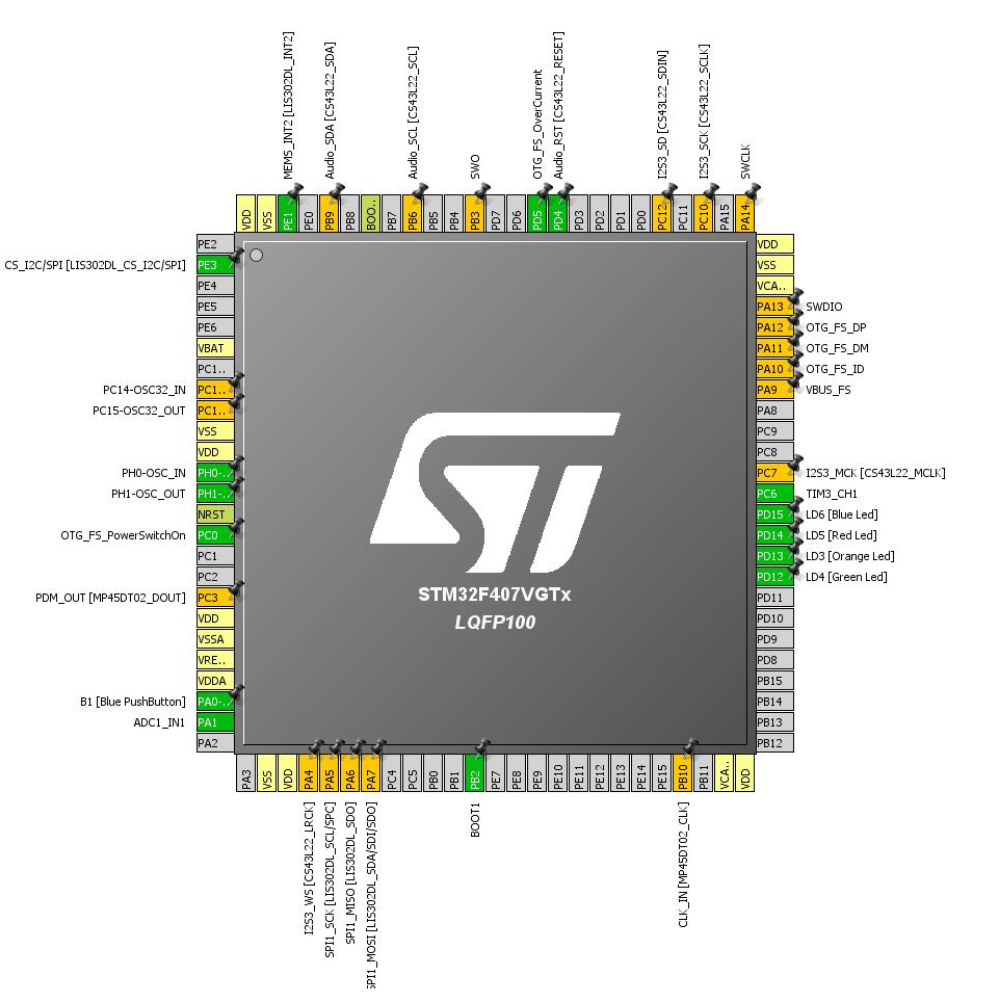
\includegraphics[scale=0.7]{./figures/pin_config.PNG}
			\caption{HAL's Visualization of the STM32F4's Pins Configuration}
		\end{center}
	\end{figure}
	\newpage
	
	
	\chapter{Theory References}
	\begin{itemize}
		\item 1. Tool, B. and Library, C. (2018). Rectifier Circuits | Diodes and Rectifiers | Electronics Textbook. [online] Allaboutcircuits.com. Available at: https://www.allaboutcircuits.com/textbook/semiconductors/chpt-3/rectifier-circuits/ [Accessed 18 Mar. 2018].
		\item 2. Justsoftwaresolutions.co.uk. (2018). Locks, Mutexes, and Semaphores: Types of Synchronization Objects | Just Software Solutions - Custom Software Development. [online] Available at: https://www.justsoftwaresolutions.co.uk/threading/locks-mutexes-semaphores.html [Accessed 18 Mar. 2018].
	\end{itemize}
\end{appendix}
\end{document}
